\begin{frame}{Problem setup}
\begin{itemize}
    \item We have access to an embedding matrix $\phi(\mathcal D) \in \mathbb R^{n \times m}$ at a certain block of the transformer residual stream.
    \item Directions in $\mathbb R^m$ correspond to various concepts.
    \item However, these directions are in superposition.
    \item Main idea: compare $\hat I (c_j)$ for various dictionary learning methods.
\end{itemize}
\end{frame}

\begin{frame}{Sparse autoencoders}
\begin{itemize}
    \item Sparse autoencoders are a dictionary-learning method that reconstruct vectors from a sparse combination of learned dictionary features.
    \item Learn dictionary $c \in \mathbb R^p$ of functions from residual stream positions $x \in \mathbb R^m$
    \item Main idea: $p > m$ so that features are {\it monosemantic}.
\end{itemize}
Model:
    \begin{align*}
        \hat x = W^T c \\
        c = \text{ReLU(Wx + b)}
    \end{align*}
    Objective function:
    \begin{align*}
        \|x - \hat x\|_2^2 + \lambda \|c\|_1
    \end{align*}
\end{frame}

\begin{frame}{Results for selected concepts}
\begin{figure}
    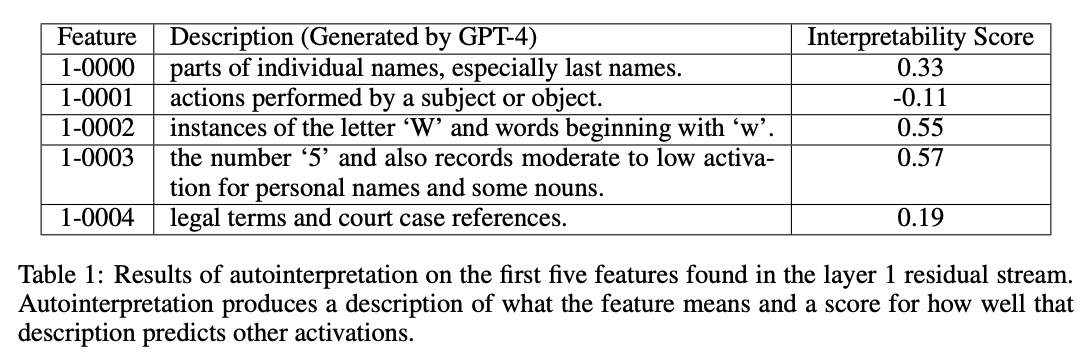
\includegraphics[width=10cm]{img/table1.png}
    \caption*{\citet{Cunningham2023-mu}}
\end{figure}
\end{frame}

\begin{frame}{Results for various dictionary learning methods}
\begin{figure}
    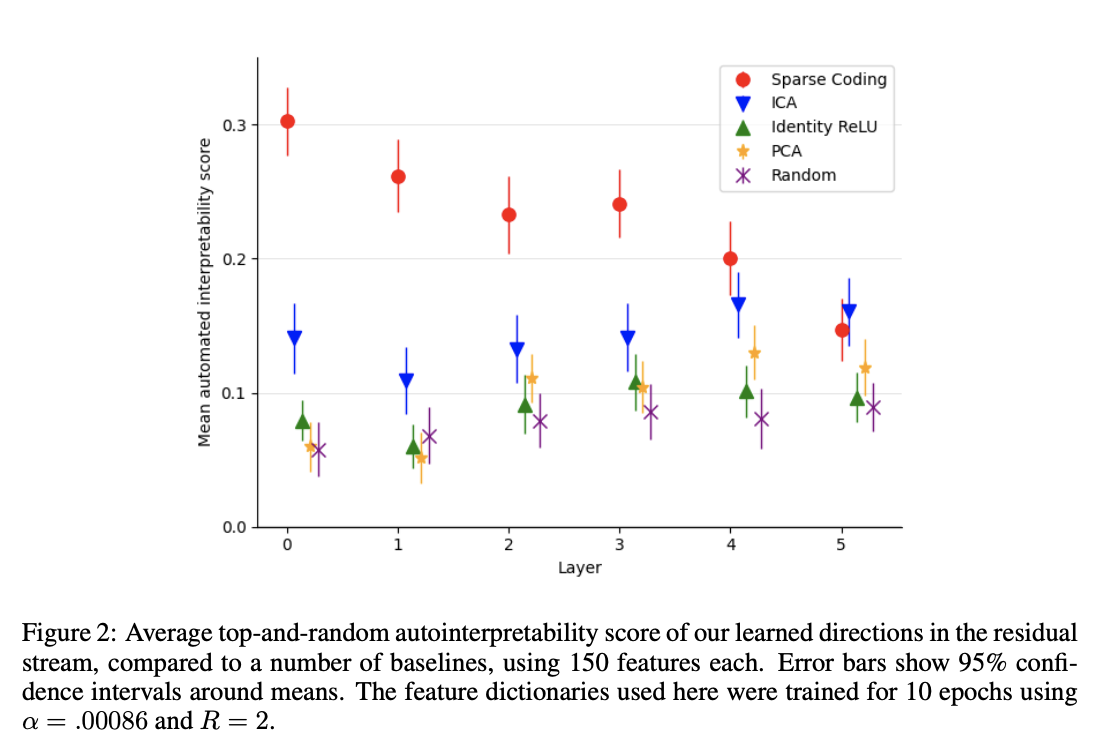
\includegraphics[width=10cm]{img/figure2.png}
    \caption*{\citet{Cunningham2023-mu}}
\end{figure}
\end{frame}

\begin{frame}{Circuit ablation study}
\begin{itemize}
\item Transformers represent {\it circuits} that correspond to complex concepts.
\item Indirect object identification \citep{Wang2022-yo}: "Then, Alice and Bob went to the store. Alice
gave a snack to \_”.
\item \citet{Conmy-undated-os} algorithm finds subset of most predictive features.
\end{itemize}
\begin{figure}
    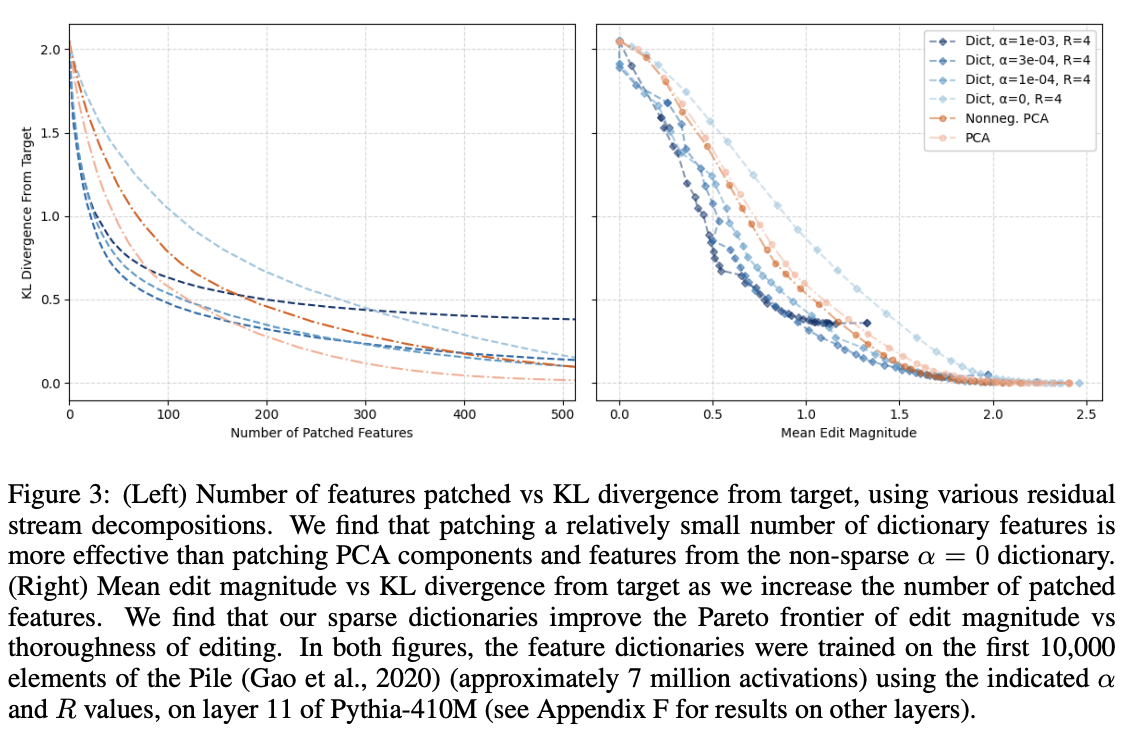
\includegraphics[width=8cm]{img/klresults.png}
\end{figure}
\end{frame}